% ================================================
% 文件: Lyonodyne-17.tex
% 章节: Lyonodyne-17 矿石收音机（经典示例）
% 所属部分: 接收机技术 -> 广播接收机
% 版本: v1.0
% ================================================
% 本节目录结构（树状）:
% \section{Lyonodyne-17 矿石收音机}
% ├── \subsection{设计原理}
% │   ├── 设计理念
% │   ├── 调谐电容器
% │   ├── 线圈设计
% │   └── 致谢
% ├── \subsection{Tuggle 前端}
% ├── \subsection{电路详情}
% │   ├── 电路结构
% │   ├── 信号路径
% │   └── 阻抗匹配
% ├── \subsection{天线系统}
% │   ├── 天线规格
% │   └── 天线调谐
% ├── \subsection{关键元件}
% │   ├── 元件清单
% │   ├── 电容器
% │   ├── 二极管
% │   ├── 线圈
% │   ├── 电阻
% │   ├── 开关
% │   ├── 变压器
% │   └── 电话机
% ├── \subsection{性能参数}
% │   ├── 整机参数
% │   ├── 线圈参数汇总
% │   └── 电容参数汇总
% ├── \subsection{比赛成绩}
% │   ├── 2001年DX比赛
% │   └── 2003年DX比赛
% ├── \subsection{技术要点}
% │   ├── 选择性vs灵敏度
% │   └── 城市vs乡村接收
% ├── \subsection{历史背景}
% │   ├── 矿石收音机DX竞赛
% │   └── 设计者Mike Tuggle
% └── \subsection{参考资料}
% ================================================

\section{Lyonodyne-17 矿石收音机}
\label{sec:lyonodyne_17}

Lyonodyne-17 是一款高级远程接收矿石收音机（DX Crystal Set），由美国夏威夷的 Mike Tuggle 设计制造。该收音机是从 1974 年开始的一系列 DX 矿石收音机演进的高级版本。Mike Tuggle 自 1959 年发现可以用矿石收音机进行 DX 接收以来，就对矿石收音机产生了浓厚兴趣。

Lyonodyne-17 是一款完全被动的接收设备——无放大器、无检波器偏置。电路采用双调谐设计，使用超高品质元件：镀银可变电容和高Q值利兹线篮绕线圈。独立线圈Q值在广播频段达到 700 以上，大部分频段超过 1000。检波器采用单个 12101 3RT 二极管（Radio Shack 销售为"1N34 型"），这是设计者目前找到的最好的检波二极管。耳机使用高品质声动力（平衡电枢式）军用剩余电话机，通过高品质线路变压器与高阻抗次级调谐电路/检波器匹配。加上陷波器等组件，整机占用大部分桌面空间。

该收音机在 2000 年和 2001 年连续两年获得 DX"Open Class"比赛第一名，2001 年创下了接收 63 个电台（包括古巴）的记录。2003 年比赛中，Mike 使用方铅矿（硫化铅）作为检波器自我限制条件后获得第二名。该收音机采用"Tuggle"前端设计和超高品质元件。

\begin{figure}[htbp]
	\centering
	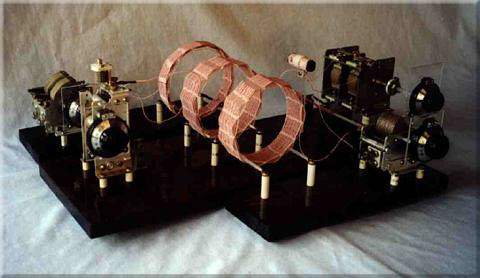
\includegraphics[width=0.7\linewidth]{Lyonodyne-17/Images/lyonodyne17b}
	\caption{Lyonodyne-17 矿石收音机}
	\label{fig:lyonodyne17}
\end{figure}

\begin{figure}[htbp]
	\centering
	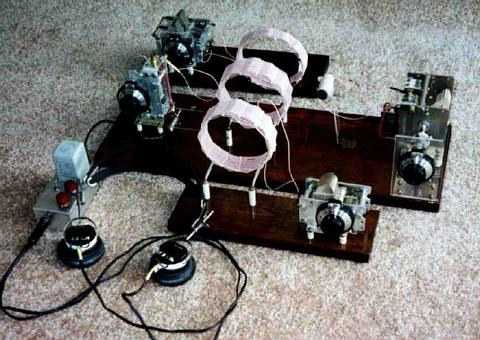
\includegraphics[width=0.8\linewidth]{Lyonodyne-17/Images/lyonodyne17d}
	\caption{Lyonodyne-17 整机实物图}
	\label{fig:lyonodyne17_full}
\end{figure}

\subsection{设计原理}
\label{subsec:lyonodyne_design_principle}

\subsubsection*{设计理念}

经过多次实验失败后，设计者得出结论：调谐电路的"高L/C比"并非关键。结合 200/46 利兹线（后改用 660/46）线圈获得的高Q值，促成了对收音机设计的重新思考。这导致了完全重建的矿石收音机——相同电路，但根据以下原则重新设计元件：

\begin{enumerate}
    \item 设计尽可能低的 L/C 比
    \item 使用最高质量的可变电容器
    \item 必要时用高质量空气微调器垫整可变电容，以获得最低频率并展开高端调谐
    \item 选择线圈设计，使Q值在广播频段中央达到峰值——接近自谐振频率工作是适得其反的
\end{enumerate}

\subsubsection*{调谐电容器}

使用了超高质量的调谐电容器（镀银，陶瓷支架）。两个主要调谐电容候选者：
\begin{itemize}[leftmargin=2cm]
    \item 500\,pF 镀银陶瓷绝缘电容
    \item 双联 470\,pF 每联镀银陶瓷绝缘电容
    \item 典型并联漏电阻测量值为 20 兆欧（Boonton 260-A 测量）
\end{itemize}

\subsubsection*{线圈设计}

线圈采用高Q值利兹线篮绕设计：
\begin{itemize}[leftmargin=2cm]
    \item 使用 660/46 利兹线
    \item 线圈直径与长度比约 5:1
    \item 采用"过1下1"绕线模式
    \item 独立线圈Q值在广播频段达到 700 以上
\end{itemize}

\subsubsection*{致谢}

作者感谢以下人士对 Lyonodyne-17 设计的贡献：

\begin{itemize}[leftmargin=2cm]
    \item \textbf{Oklahoma 的 Bill Bowers}：向作者介绍了用于中频的细股利兹线的优点，以及使用比理论建议更大的线圈直径与长度比（约 5:1），并建议回归"过1下1"绕线模式。虽然这种绕线模式不如作者多年使用的"过2下1"模式美观，电感值也较低，但Q值确实显著更高。
    \item \textbf{Al Klase}：长期大力宣传声动力电话机的优点，最终作者不得不听取建议——尽管作者曾坚信没有任何东西能超越 Brush 矿石电话机。声动力电话机确实令人耳目一新，性能提升了一个数量级。
\end{itemize}

\subsection{Tuggle 前端}
\label{subsec:tuggle_frontend}

Lyonodyne-17 采用了"Tuggle"前端设计，这是一种经过优化的双调谐电路结构，具有极高的选择性和灵敏度。Tuggle 前端是 Mike Tuggle 多年实验的成果，结合了低 L/C 比设计、高Q值元件和精密耦合控制等先进技术。

\begin{figure}[htbp]
	\centering
	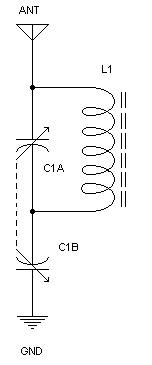
\includegraphics[width=\linewidth]{Lyonodyne-17/Images/tugglefrontend.png}
	\caption{Tuggle 前端电路图}
	\label{fig:tuggle_frontend}
\end{figure}

Tuggle 前端的核心特点：
\begin{itemize}[leftmargin=2cm]
    \item 双调谐电路设计，初级和次级独立调谐
    \item 松耦合设计，减少相互影响
    \item 高Q值线圈和电容，保证灵敏度和选择性
    \item 精密耦合控制，陷波器耦合保持最小
    \item 能够接收紧邻强本地信号的相邻频率电台
\end{itemize}

\subsection{电路详情}
\label{subsec:lyonodyne_circuit}

\subsubsection*{电路结构}

Lyonodyne-17 采用双调谐电路设计：

\begin{itemize}[leftmargin=2cm]
    \item \textbf{初级调谐（天线-地线系统）}：由 L1-C1 调谐
    \item \textbf{次级调谐（检波器）}：由 L2-C2 调谐
    \item \textbf{耦合方式}：通过 L1-L2 松耦合（物理距离 3--4 英寸）
    \item \textbf{线圈放置}：L1 和 L2 径向放置（并排）
    \item \textbf{干扰陷波器}：两个高Q值并联 L-C 电路，线圈轴向耦合到 L2
\end{itemize}

L1 对 L2-C2 的调谐和Q值几乎没有影响，但 QRM 陷波器会影响调谐，特别是在 QRM 频率附近。因此，陷波器的耦合保持在最小程度，同时仍然允许接收感兴趣的电台。该收音机能够接收紧邻强本地信号的相邻频率电台。

\begin{figure}[htbp]
	\centering
	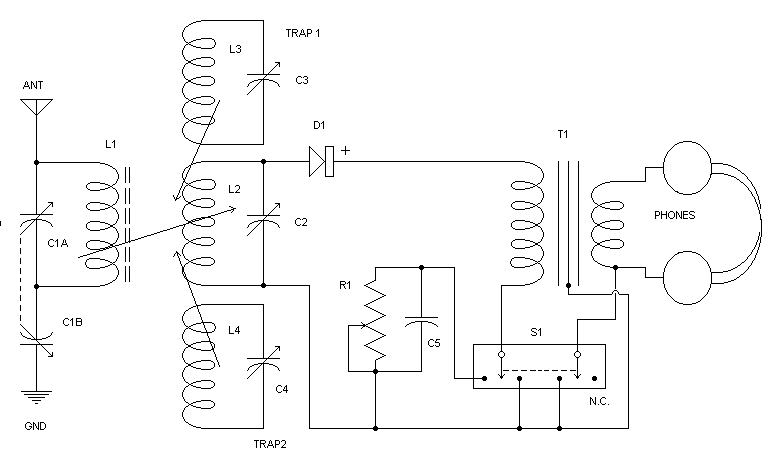
\includegraphics[width=\linewidth]{Lyonodyne-17/Images/lyonodyne17schematicb.png}
	\caption{Lyonodyne-17 整机电路图}
	\label{fig:lyonodyne17_schematic}
\end{figure}

\subsubsection*{信号路径}

\begin{enumerate}
    \item 天线接收信号，由初级 L1-C1 调谐
    \item 通过松耦合传递到次级 L2-C2
    \item 干扰陷波器滤除强干扰信号
    \item 检波器（12101 3RT 二极管）解调信号
    \item 通过 UTC A-27 变压器匹配到声动力电话机
\end{enumerate}

\subsubsection*{阻抗匹配}

\begin{itemize}[leftmargin=2cm]
    \item 检波器正向电阻估计约 200\,k$\Omega$
    \item 使用 UTC A-27 100\,k$\Omega$ 到 200\,$\Omega$ 输入变压器
    \item 声动力电话机低阻抗，通过变压器与次级调谐电路匹配
    \item 这种阻抗配置允许检波器-电话机直接跨接在调谐电路上，不会过度加载
\end{itemize}

过去使用抽头的方式非常麻烦——特别是在利兹线上。更重要的是，抽头会降低线圈的Q值，应尽可能避免使用。

\subsection{天线系统}
\label{subsec:lyonodyne_antenna}

\subsubsection*{天线规格}

\begin{itemize}[leftmargin=2cm]
    \item 类型：50 英尺，4 线平顶天线
    \item 线间距：1 英尺
    \item 高度：约 25 英尺
    \item 接地：直接接入城市供水系统
\end{itemize}

作者之前使用过 105 英尺长的长线天线，但大风刮倒了另一端的树木。较短的平顶天线效果很好，因此作者将其带到了夏威夷，在那里长天线的空间非常宝贵。这个天线几乎是作者能在这片土地上合理安装的最大尺寸了。

\subsubsection*{天线调谐}

天线-地线系统可通过初级 L1-C1 调谐至谐振，提高灵敏度和选择性。

\subsection{关键元件}
\label{subsec:lyonodyne_components}

\subsubsection*{元件清单（截至 2001年2月5日）}

\paragraph{电容器}

\begin{itemize}[leftmargin=2cm]
    \item \textbf{C1}：双联可变电容，每联 15--470\,pF，高并联漏电阻（Rp）
    \item \textbf{C2}：R/C（或 TRW）15--497\,pF 直线频率可变电容，Rp约20兆欧。型号 No.\,107-C-522；FSN\,5910-546-9239；Fair Radio Sales 目录号 C123/URM125
    \item \textbf{C3}：同 C2
    \item \textbf{C4}：同 C2
    \item \textbf{C5}：0.02\,$\mu$F 聚苯乙烯电容
\end{itemize}

\paragraph{二极管}

\begin{itemize}[leftmargin=2cm]
    \item \textbf{D1}：经过听音筛选的 Radio Shack 12101 3RT 锗二极管
\end{itemize}

\paragraph{线圈}

\begin{verbatim}
L1 51 turns 100/44 litz on 5/8" dia. x 1-3/16" long ferrite rod, u(eff) = 10.33;
length = 1-35/64"; L = 146.6 uH; Co = 4.54 pF; Q @ 0.5 MHz = 649

L2 36 turns 660/46 litz, basket-wound over-1, under-1 on 5" dia. 13-point form;
 length = 1.9375"; L = 185.6 uH; Co = 7.40 pF; Q @ 0.8 MHz = 1134

L3 36 turns 660/46 litz, basket-wound over-1, under-1 on 5" dia. 13-point form;
 length = 1.9375"; L = 185.7 uH; Co = 7.40 pF; Q @ 0.8 MHz = 1060

L4 42 turns 660/46 litz, basket-wound over-1, under-1 on 4-1/4" dia. 13-point form; length = 2.25".  L= 186.7 uH; Co = 6.45 pF; Q @ 0.8 MHz = 1082
\end{verbatim}

\begin{itemize}[leftmargin=2cm]
    \item \textbf{L1}（初级调谐线圈）：51匝 100/44 利兹线，绕在铁氧体棒上，$\mu_{\rm eff}$ = 10.33，L = 146.6\,$\mu$H，Q @ 0.5\,MHz = 649
    \item \textbf{L2}（次级调谐线圈）：36匝 660/46 利兹线，篮绕"过1下1"，L = 185.6\,$\mu$H，Q @ 0.8\,MHz = 1134
    \item \textbf{L3}（陷波器线圈）：36匝 660/46 利兹线，篮绕"过1下1"，L = 185.7\,$\mu$H，Q @ 0.8\,MHz = 1060
    \item \textbf{L4}（陷波器线圈）：42匝 660/46 利兹线，篮绕"过1下1"，L = 186.7\,$\mu$H，Q @ 0.8\,MHz = 1082
\end{itemize}

\paragraph{电阻}

\begin{itemize}[leftmargin=2cm]
    \item \textbf{R1}：500\,k$\Omega$ 电位器
\end{itemize}

\paragraph{开关}

\begin{itemize}[leftmargin=2cm]
    \item \textbf{S1}：DPDT 微型拨动开关
\end{itemize}

\paragraph{变压器}

\begin{itemize}[leftmargin=2cm]
    \item \textbf{T1}：UTC A-27 输入变压器，初级 100\,k$\Omega$；次级抽头 50--600\,$\Omega$——使用 RCA 电话机时，约 200\,$\Omega$ 效果最佳
\end{itemize}

\paragraph{电话机}

\begin{itemize}[leftmargin=2cm]
    \item \textbf{PHONES}：RCA MI-2045 声动力电话机，业内称为"Big Cans"
\end{itemize}

\paragraph{备注}

所有可变电容都配备游标驱动刻度盘，便于精细调谐。

\subsection{性能参数}
\label{subsec:lyonodyne_performance}

\subsubsection*{整机参数}

\begin{table}[htbp]
    \centering
    \caption{Lyonodyne-17 整机性能参数}
    \label{tab:lyonodyne_performance}
    \begin{tabular}{lp{8cm}}
        \toprule
        \textbf{参数} & \textbf{数值} \\
        \midrule
        独立线圈Q值 & 700+（广播频段） \\
        部分频段Q值 & 1000+ \\
        频率范围 & AM 广播频段（540--1600\,kHz） \\
        选择性 & 高（双调谐+陷波器） \\
        灵敏度 & 极高（高Q值元件） \\
        电源需求 & 无（完全被动） \\
        电路类型 & 双调谐被动矿石收音机 \\
        检波器类型 & 锗二极管（12101 3RT） \\
        耳机类型 & 声动力电话机（平衡电枢式） \\
        \bottomrule
    \end{tabular}
\end{table}

\subsubsection*{线圈参数汇总}

\begin{table}[htbp]
    \centering
    \caption{Lyonodyne-17 线圈参数}
    \label{tab:lyonodyne_coils}
    \begin{tabular}{llllll}
        \toprule
        \textbf{线圈} & \textbf{匝数} & \textbf{线规} & \textbf{骨架直径} & \textbf{电感} & \textbf{Q值} \\
        \midrule
        L1 & 51 & 100/44 litz & 5/8"（铁氧体棒） & 146.6\,$\mu$H & 649 @ 0.5\,MHz \\
        L2 & 36 & 660/46 litz & 5"（13点骨架） & 185.6\,$\mu$H & 1134 @ 0.8\,MHz \\
        L3 & 36 & 660/46 litz & 5"（13点骨架） & 185.7\,$\mu$H & 1060 @ 0.8\,MHz \\
        L4 & 42 & 660/46 litz & 4-1/4"（13点骨架） & 186.7\,$\mu$H & 1082 @ 0.8\,MHz \\
        \bottomrule
    \end{tabular}
\end{table}

\subsubsection*{电容参数汇总}

\begin{table}[htbp]
    \centering
    \caption{Lyonodyne-17 电容参数}
    \label{tab:lyonodyne_capacitors}
    \begin{tabular}{lll}
        \toprule
        \textbf{电容} & \textbf{容量范围} & \textbf{备注} \\
        \midrule
        C1 & 15--470\,pF（双联） & 高并联漏电阻 \\
        C2 & 15--497\,pF & R/C/TRW，Rp约20兆欧 \\
        C3 & 15--497\,pF & 同 C2 \\
        C4 & 15--497\,pF & 同 C2 \\
        C5 & 0.02\,$\mu$F & 聚苯乙烯电容 \\
        \bottomrule
    \end{tabular}
\end{table}

\subsection{比赛成绩}
\label{subsec:lyonodyne_competition}

\subsubsection*{2001 年 DX 比赛}

\begin{itemize}[leftmargin=2cm]
    \item 名次：第一名（Open Class）
    \item 接收电台数：63 个
    \item 最远接收：古巴
    \item 全部在 AM 广播频段接收
\end{itemize}

\subsubsection*{2003 年 DX 比赛}

\begin{itemize}[leftmargin=2cm]
    \item 名次：第二名
    \item 特殊条件：使用方铅矿（硫化铅）作为检波器
    \item 自我限制条件，展示技术实力
\end{itemize}

\subsection{技术要点}
\label{subsec:lyonodyne_technical_points}

\subsubsection*{选择性 vs 灵敏度}

矿石收音机 DX 接收面临两个主要问题：
\begin{itemize}[leftmargin=2cm]
    \item \textbf{选择性}：分离强本地电台，接收弱信号
    \item \textbf{灵敏度}：接收微弱信号的能力
\end{itemize}

Lyonodyne-17 通过以下设计平衡这两个需求：
\begin{itemize}[leftmargin=2cm]
    \item 双调谐电路提高选择性
    \item 高Q值元件保证灵敏度
    \item 干扰陷波器滤除强干扰
    \item 松耦合设计减少相互影响
\end{itemize}

\subsubsection*{城市 vs 乡村接收}

\begin{itemize}[leftmargin=2cm]
    \item \textbf{城市环境}：需要高选择性分离强本地电台
    \item \textbf{乡村环境}：可以"宽开"接收弱信号
    \item Lyonodyne-17 设计兼顾两种环境
\end{itemize}

\subsection{历史背景}
\label{subsec:lyonodyne_history}

\subsubsection*{矿石收音机 DX 竞赛}

矿石收音机 DX 竞赛是无线电爱好者的重要活动，挑战在完全被动的条件下接收最远的电台。Lyonodyne-17 的成功展示了矿石收音机技术的巅峰。

\subsubsection*{设计者 Mike Tuggle}

\begin{itemize}[leftmargin=2cm]
    \item 自 1959 年开始对矿石收音机感兴趣
    \item 多年实验经验
    \item 开发了多款高性能矿石收音机
    \item Lyonodyne 系列从 1974 年开始演进
\end{itemize}

\subsection{参考资料}
\label{subsec:lyonodyne_references}

\begin{itemize}[leftmargin=2cm]
    \item Crystal Radio DXing：\url{https://www.qsl.net/ve7sl/crystal.html}
    \item Boyd House Crystal Radio：\url{https://www.boydhouse.com/darryl/crystalradio.net/crystalsets/lyonodyne/index.shtml}
\end{itemize}
